\documentclass[
	12pt,
	]{article}
		\usepackage{xcolor}
			\usepackage[dvipsnames]{xcolor}
			\usepackage[many]{tcolorbox}
		\usepackage{changepage}
		\usepackage{titlesec}
		\usepackage{mdframed}
		\usepackage{mathtools, amssymb, amsfonts, amsthm, bm,amsmath} 
		\usepackage{array, tabularx, booktabs}
		\usepackage{graphicx,wrapfig, float, caption}
		\usepackage{tikz,physics,cancel, siunitx, xfrac}
		\usepackage{graphics, fancyhdr}
		\usepackage{lipsum}
		\usepackage{xparse}
		\usepackage{thmtools}
		\usepackage{mathrsfs}
		\usepackage{undertilde}
		\usepackage{dutchcal}
		\usepackage{tikz}
		\usepackage{fullpage}
		\usepackage[labelfont=bf]{caption}
	\newcommand{\td}{\text{dim}}
	\newcommand{\tvw}{T : V\xrightarrow{} W }
	\newcommand{\ttt}{\widetilde{T}}
	\newcommand{\ex}{\textbf{Example}}
	\newcommand{\aR}{\alpha \in \mathbb{R}}
	\newcommand{\abR}{\alpha \beta \in \mathbb{R}}
	\newcommand{\un}{u_1 , u_2 , \dots , n}
	\newcommand{\an}{\alpha_1, \alpha_2, \dots, \alpha_2 }
	\newcommand{\sS}{\text{Span}(\mathcal{S})}
	\newcommand{\sSt}{($\mathcal{S}$)}
	\newcommand{\la}{\langle}
	\newcommand{\ra}{\rangle}
	\newcommand{\Rn}{\mathbb{R}^{n}}
	\newcommand{\R}{\mathbb{R}}
	\newcommand{\Rm}{\mathbb{R}^{m}}
	\usepackage{fullpage}
	


	\usepackage{mathtools}
	\DeclarePairedDelimiter{\norm}{\lVert}{\rVert}
	\newcommand{\vectorproj}[2][]{\textit{proj}_{\vect{#1}}\vect{#2}}
	\newcommand{\vect}{\mathbf}
	\newcommand{\uuuu}{\sum_{i=1}^{n}\frac{<u,u_i}{<u_i,u_i>} u_i}
	\newcommand{\B}{\mathcal{B}}
	\newcommand{\Ss}{\mathcal{S}}
	
	\newtheorem{theorem}{Theorem}[section]
	\theoremstyle{definition}
	\newtheorem{corollary}{Corollary}[theorem]
	\theoremstyle{definition}
	\newtheorem{lemma}[theorem]{Lemma}
	\theoremstyle{definition}
	\newtheorem{definition}{Definition}[section]
	\theoremstyle{definition}
	\newtheorem{Proposition}{Proposition}[section]
	\theoremstyle{definition}
	\newtheorem*{example}{Example}
	\theoremstyle{example}
	\newtheorem*{note}{Note}
	\theoremstyle{note}
	\newtheorem*{remark}{Remark}
	\theoremstyle{remark}
	\newtheorem*{example2}{External Example}
	\theoremstyle{example}
	
	\title{PHYS241 Assignment 4.}
	\titleformat*{\section}{\LARGE\normalfont\fontsize{12}{12}\bfseries}
	\titleformat*{\subsection}{\Large\normalfont\fontsize{10}{15}\bfseries}
	\author{Mihail Anghelici 260928404}
	\date{\today}
	
	\relpenalty=9999
		\binoppenalty=9999
	
		\renewcommand{\sectionmark}[1]{%
		\markboth{\thesection\quad #1}{}}
		
		\fancypagestyle{plain}{%
		  \fancyhf{}
		  \fancyhead[L]{\rule[0pt]{0pt}{0pt} Assignment $4$} 
		  \fancyhead[R]{\small Mihail Anghelici $260928404$} 
		  \fancyfoot[C]{-- \thepage\ --}
		  \renewcommand{\headrulewidth}{0.4pt}}
		\pagestyle{plain}
		\setlength{\headsep}{1cm}
		
	\begin{document}
	\maketitle
		\section*{Question 1.}
			\subsection*{a) }
				The conductor has an induced f.e.m with current in opposite direction therefore voltage conservation across the circuit gives
				\begin{gather*}
					\frac{Q}{C} + L\dv{I}{t} + RI = 0 \xrightarrow{d/dt} \frac{1}{C}I + L\dv[2]{I}{t}+ R\dv{I}{t} =0 
					\intertext{Dividing by $L$ and since $dQ/dt$ in this set-up equals $I$ , }
					\therefore \dv[2]{I}{t} + \Gamma \dv{I}{t} + \omega_{0}^{2}I = 0.
				\end{gather*}
				Homogeneous second order differential equations, let us find the roots to have a solution.
				\begin{gather*}
					\implies \frac{-\Gamma \pm \sqrt{\Gamma^{2} -4\omega_{0}^{2}}}{2} = \frac{-\Gamma}{2} \pm \sqrt{\left(\frac{-\Gamma}{2}\right)^{2} -\omega_{0}^{2}} 
				\end{gather*}
				Since we're only interested in the undamped case , the solutions are of complex form with $I(t) = -\frac{\Gamma}{2} \pm j\omega_{f}$. So we have the general solution, 
				\begin{align*}
				 I(t) &= c_{1}e^{-\left(\frac{\Gamma}{2} - j\omega_{f}\right)t} + c_{2}e^{\left(\frac{-\Gamma}{2}+j\omega_{f}\right)t},\\
				 &=e^{\frac{-\Gamma}{2}t}\left(A\cos \omega_{f}t + B\sin \omega_{f}t\right).
				 \end{align*}
				 Let us find the initial conditions $A$ and $B$.
				 \begin{gather*}
				 	\text{The current in the circuit is initially $0$} \  \implies \ A = 0. \\
				 	\text{Relating voltage conservation to current gives } \ \frac{Q}{C} + L\dv{I}{t}+RI = 0 
				 	\intertext{At $t=0$ the current is $0$ therefore and $Q(0) = C V_{0}$,}
				 	\frac{Q}{C} = -L\dv{I}{t} \implies -V_{0} = L\dv{I}{t} \implies B = \frac{-V_{0}}{L\omega_{f}}.
 				 \end{gather*}
 				 The general solution is therefore 
 				 $$ I(t) = \frac{-V_{0}}{\omega_{f}L}e^{\frac{-\Gamma}{2}t}\sin \omega_{f}t.$$
 				\subsection*{b) }
 					Since $Q(t) = \int_{0}^{t}I(t') \ dt'$ and $\Delta V_{C} (t) = Q(t)/C$, it follows that 
 					\begin{align*}
 					 \Delta V_{C}(t) &= \frac{1}{C}\int_{0}^{t}I(t')\ dt'.\\
 					 &=\left(\frac{1}{C}\right)\int_{0}^{t}\frac{-V_{0}}{\omega_{f}L}e^{\frac{-\Gamma}{2}}\sin \omega_{f}t \ dt
 					 \intertext{Applying integral by parts twice with $u = e^{\frac{-\Gamma}{2}t}$ and $dv = \sin \omega_{f}t$, we obtain}
 					 &=\left(\frac{V_{0}}{C\omega_{f}L}\right)\left(\frac{\frac{e^{\frac{-\Gamma}{2}t}}{\omega_{f}}\left(-\cos\omega_{f}-\frac{\Gamma\sin\omega_{f}t}{2\omega_{f}}\right)}{\left(1+\frac{\Gamma^{2}}{4\omega_{f}^{2}}\right)}\right)\\
 					 &=\left(\frac{-V_{0}}{LC}\right)\frac{4e^{\frac{-\Gamma}{2}t}\left(-\cos\omega_{f}t-\frac{\Gamma\sin\omega_{f}t}{2\omega_{f}}\right)}{(4\omega_{f}^{2}+\Gamma^{2})}.
 					\end{align*}
 				\subsection*{c) }
 					Let us verify that the voltage drop across the capacitor converges to $0$ as $t \to \infty$.
 					\begin{gather*}
 						\lim\limits_{t\to\infty} \left(\frac{-V_{0}}{LC}\right)\frac{4e^{\frac{-\Gamma}{2}t}\left(-\cos\omega_{f}t-\frac{\Gamma\sin\omega_{f}t}{2\omega_{f}}\right)}{(4\omega_{f}^{2}+\Gamma^{2})}\\ = \left(\frac{-V_{0}}{(LC)(4\omega_{f}^{2}+\Gamma^{2})}\right) \lim\limits_{t \to \infty} 4e^{\frac{-\Gamma}{2}t}\left(-\cos\omega_{f}t-\frac{\Gamma\sin\omega_{f}t}{2\omega_{f}}\right) = 0.
 						\intertext{Since indeed $e^{-\Gamma t/ 2}$ converges to $0$ while the waves just oscillate.}
 						\therefore \checkmark
 					\end{gather*}
		\section*{Question 2.}
			Let us take the derivative with respect to $x$ and set equal to zero to find the maximal value.
			\begin{align*}
				\abs{\frac{\widetilde{\Delta V_{C}}}{\widetilde{V}}} = \frac{1}{\sqrt{\left(1-\frac{\omega^{2}}{\omega_{0}^{2}}\right)^{2} + (\omega \tau )^{2}}} 
				\intertext{Taking the derivative and setting equal to 0 we get }
				2\tau^{2}\omega - \frac{4\omega \left(1-\frac{\omega^{2}}{\omega_{0}^{2}}\right)^{2}}{\omega_{0}^{2}} = 0 
			\end{align*}
			\begin{gather*}
				\implies \omega_{0}^{4}\tau^{2} \omega -2\omega (\omega_{0}^{2} - \omega^{2}) = 0 \implies 
				\omega(\omega_{0}^{4} \tau^{2} - 2(\omega_{0}^{2} - \omega^{2})) = 0
				\intertext{$\omega \neq 0$ for the largest value }
				\omega_{0}^{4} \tau^{2} - 2(\omega_{0}^{2} - \omega^{2}) = 0 
				\implies 2\omega^{2} = 2\omega_{0}^{2} - \omega_{0}^{4} \tau^{2} \\
				\therefore \omega = \omega_{0}\pm \sqrt{1- \frac{\omega_{0}^{2} \tau^{2}}{2}}.
 			\end{gather*}
 		\section*{Question 3.}
 			\subsection*{a) }
 				Let us find the equivalent impedence, 
 				\begin{gather*}
 					\frac{1}{Z_{2}} = \left(\frac{1}{j\omega L} + j\omega C\right)^{-1} \implies Z_{2} = \frac{j\omega L}{1-\omega^{2} L C} ,  \\
 					\therefore Z_{\text{eq}} = R + \frac{j\omega L}{1-\omega^{2} L C}.
 				\end{gather*}
 				We may now find simplify an expression for the current, 
 				\begin{gather*}
 					\widetilde{I} = \frac{V_{0} e^{j\omega t}}{R + \frac{j\omega L}{1-\omega^{2} L C}} = \left(\frac{V_{0}}{R}\right) \frac{j\omega\tau}{j\omega\tau - \frac{\sfrac{\omega^{2}}{\omega_{0}^{2}}}{1-\sfrac{\omega^{2}}{\omega_{0}^{2}} }} e^{j\omega t}
 				\end{gather*}
 				Let us find the amplitude of the previous expression 	
 				\begin{gather*}
 					\abs{\widetilde{I}}^{2} = \left(\frac{V_{0}}{R}\right)^{2}\left(\frac{j\omega\tau}{j\omega\tau - \frac{\sfrac{\omega^{2}}{\omega_{0}^{2}}}{1-\sfrac{\omega^{2}}{\omega_{0}^{2}} }}\right)\left(\frac{-j\omega\tau}{-j\omega\tau - \frac{\sfrac{\omega^{2}}{\omega_{0}^{2}}}{1-\sfrac{\omega^{2}}{\omega_{0}^{2}} }} \right) = \left(\frac{V_{0}}{R}\right)^{2}\frac{(\omega\tau)^{2}}{(\omega\tau)^{2} + \left(\frac{\sfrac{\omega^{2}}{\omega_{0}^{2}}}{1-\sfrac{\omega^{2}}{\omega_{0}^{2}}}\right)^{2}} \\
 					\implies \abs{\widetilde{I}} = \left(\frac{V_{0}}{R}\right)\frac{\omega\tau}{\sqrt{(\omega\tau)^{2} + \left(\frac{\sfrac{\omega^{2}}{\omega_{0}^{2}}}{1-\sfrac{\omega^{2}}{\omega_{0}^{2}}}\right)^{2}}}.
 				\end{gather*}
 				Let us now find the phase offset of the complex current, 
 				\begin{align*}
 					\widetilde{I} &= \frac{\widetilde{V}}{R} \frac{j\omega\tau}{j\omega\tau - \frac{\sfrac{\omega^{2}}{\omega_{0}^{2}}}{1-\sfrac{\omega^{2}}{\omega_{0}^{2}}}} = \frac{\widetilde{V}}{R}\left(\frac{j\omega\tau}{j\omega\tau - \frac{\sfrac{\omega^{2}}{\omega_{0}^{2}}}{1-\sfrac{\omega^{2}}{\omega_{0}^{2}}}}\right)\left(\frac{-j\omega\tau - \frac{\sfrac{\omega^{2}}{\omega_{0}^{2}}}{1-\sfrac{\omega^{2}}{\omega_{0}^{2}}}}{-j\omega\tau -\frac{\sfrac{\omega^{2}}{\omega_{0}^{2}}}{1-\sfrac{\omega^{2}}{\omega_{0}^{2}}}}\right) \\
 					\implies Z_{\text{Numerator}} &= (\omega\tau)^{2} - j\omega\tau\left(\frac{\sfrac{\omega^{2}}{\omega_{0}^{2}}}{1-\sfrac{\omega^{2}}{\omega_{0}^{2}}}\right) \implies \phi = \tan^{-1} \left(\frac{\omega\tau\left(\frac{-\sfrac{\omega^{2}}{\omega_{0}^{2}}}{1-\sfrac{\omega^{2}}{\omega_{0}^{2}}}\right)}{(\omega\tau)^{2}}\right) \\
 					& \quad \therefore \phi = \tan^{-1}\left(\frac{\frac{-\sfrac{\omega^{2}}{\omega_{0}^{2}}}{1-\sfrac{\omega^{2}}{\omega_{0}^{2}}}}{\omega\tau}\right)
 				\end{align*}
 				Finally, we have an expression for the current inside the circuit 
 				\begin{equation*}
 					I = \left(\frac{V_{0}}{R}\right)\frac{\omega\tau}{\sqrt{(\omega\tau)^{2} + \left(\frac{\sfrac{\omega^{2}}{\omega_{0}^{2}}}{1-\sfrac{\omega^{2}}{\omega_{0}^{2}}}\right)^{2}}} e^{j(\omega t + \phi)}\quad, \text{where } \phi = \tan^{-1}\left(\frac{\frac{-\sfrac{\omega^{2}}{\omega_{0}^{2}}}{1-\sfrac{\omega^{2}}{\omega_{0}^{2}}}}{\omega\tau}\right).
 				\end{equation*}
 			\subsection*{b) }
 				\begin{figure}[h]
 					\centering
 					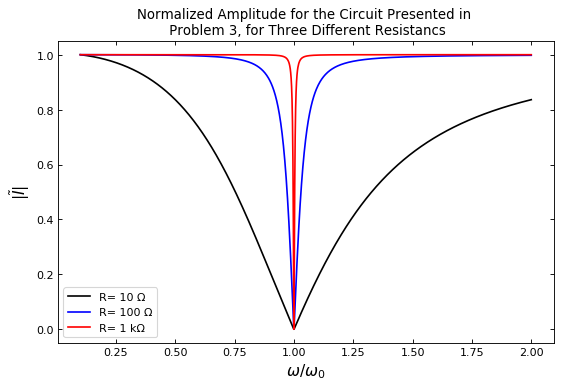
\includegraphics[width=0.8\linewidth]{PHYS241_Ass4_Figure1.png}
 					\caption{Plot of the current's amplitude found in Question 2, for three resistor configurations $R$. We note that increasing the value for the resistance in return increases the narrowness around the resonance point.}
 				\end{figure}
 		\section*{Question 4.}
 			\subsection*{a) }
 				Let us find the equivalent impedance in sub portion of the rightward side of the given circuit.
 				\begin{gather*}
 					Z_1 = j\omega L + r \qquad Z_{2} = \frac{1}{j\omega C} \\
 					Z_{||} =\left(\frac{1}{j\omega L} + j\omega C\right)^{-1} \\
 					\therefore Z_{||}= \frac{(j\omega L + r)}{1+ (j\omega L +r)j\omega C} = \frac{j\omega L +r }{1- \frac{\omega^{2}}{\omega_{0}^{2}} + j\omega C r}
 				\end{gather*}
 			\subsection*{b) }
 				\begin{equation*}
 					Z_{\text{eq}} = R + \frac{j\omega L +r }{1- \frac{\omega^{2}}{\omega_{0}^{2}} + j\omega C r}.
 				\end{equation*}
 				We may now find an expression for the current,
 				\begin{gather*}
 					\widetilde{I} = \frac{V_{0}e^{j\omega t}}{R + \frac{j\omega L +r }{1- \sfrac{\omega^{2}}{\omega_{0}^{2}} + j\omega C r}} = \left(\frac{V_{0}}{R}\right) \frac{j\omega \tau}{j\omega \tau + \frac{\sfrac{-\omega^{2}}{\omega_{0}^{2}} + j\omega C r}{1 - \sfrac{\omega^{2}}{\omega_{0}^{2}} + j\omega C r}}.
 				\end{gather*}
 				Now we find the amplitude of the previous expression
 				\begin{gather*}
 					\abs{\widetilde{I}}^{2} = \left(\frac{V_{0}}{R}\right)^{2} \left( \frac{j\omega \tau}{j\omega \tau + \frac{\sfrac{-\omega^{2}}{\omega_{0}^{2}} + j\omega C r}{1 - \sfrac{\omega^{2}}{\omega_{0}^{2}} + j\omega C r}}\right)\left( \frac{-j\omega \tau}{-j\omega \tau + \frac{\sfrac{-\omega^{2}}{\omega_{0}^{2}} -j\omega C r}{1 - \sfrac{\omega^{2}}{\omega_{0}^{2}} -j\omega C r}}\right) \\
 					 = \left(\frac{V_{0}}{R}\right)^{2} \frac{(\omega\tau)^{2}}{(\omega\tau)^{2} + \frac{(\omega C r)^{2} + \left(\frac{\omega}{\omega_{0}}\right)^{4}}{\left(1-\left(\frac{\omega}{\omega_{0}}\right)^{2}\right)^{2} + (\omega C r)^{2}}} \ \ \therefore \abs{\widetilde{I}} = \left(\frac{V_{0}}{R}\right) \frac{\omega\tau}{\sqrt{(\omega\tau)^{2} + \frac{(\omega C r)^{2} + \left(\frac{\omega}{\omega_{0}}\right)^{4}}{\left(1-\left(\frac{\omega}{\omega_{0}}\right)^{2}\right)^{2} + (\omega C r)^{2}}}}.
 				\end{gather*}
 				The current's amplitude is found and the problem is done, let us nevertheless find a complete expression for the current, we find the offset
 				\begin{gather*}
 					\widetilde{I} = \frac{\widetilde{V}}{R} \left(\frac{j\omega \tau}{j\omega \tau + \frac{\sfrac{-\omega^{2}}{\omega_{0}^{2}} + j\omega C r}{1 - \sfrac{\omega^{2}}{\omega_{0}^{2}} + j\omega C r}}\right)\left(\frac{-j\omega \tau + \frac{\sfrac{-\omega^{2}}{\omega_{0}^{2}} - j\omega C r}{1 - \sfrac{\omega^{2}}{\omega_{0}^{2}} - j\omega C r}}{-j\omega \tau + \frac{\sfrac{-\omega^{2}}{\omega_{0}^{2}} -j\omega C r}{1 - \sfrac{\omega^{2}}{\omega_{0}^{2}} - j\omega C r}}\right) \\
 					\implies Z_{\text{Numerator }} = (\omega \tau)^{2} + j\omega\tau \left(\frac{\sfrac{-\omega^{2}}{\omega_{0}^{2}} -j\omega C r}{1 - \sfrac{\omega^{2}}{\omega_{0}^{2}} - j\omega C r}\right) \\ \implies \phi = \tan^{-1} \left(\frac{\omega\tau \left(\frac{\sfrac{-\omega^{2}}{\omega_{0}^{2}} -j\omega C r}{1 - \sfrac{\omega^{2}}{\omega_{0}^{2}} - j\omega C r}\right)}{(\omega\tau)^{2}}\right) \ \ \therefore \phi = \tan^{-1}\left(\frac{\frac{\sfrac{-\omega^{2}}{\omega_{0}^{2}} -j\omega C r}{1 - \sfrac{\omega^{2}}{\omega_{0}^{2}} - j\omega C r}}{\omega\tau}\right).
 				\end{gather*}
 				Finally, we have an expression for the current inside the cirucit ,
 				\begin{equation*}
 					I = \left(\frac{V_{0}}{R}\right) \frac{\omega\tau}{\sqrt{(\omega\tau)^{2} + + \frac{(\omega C r)^{2} + \left(\frac{\omega}{\omega_{0}}\right)^{4}}{\left(1-\left(\frac{\omega}{\omega_{0}}\right)^{2}\right)^{2} + (\omega C r)^{2}}}}e^{j(\omega t + \phi)}, \ \ \ \text{where  } \phi = \tan^{-1}\left(\frac{\frac{\sfrac{-\omega^{2}}{\omega_{0}^{2}} -j\omega C r}{1 - \sfrac{\omega^{2}}{\omega_{0}^{2}} - j\omega C r}}{\omega\tau}\right).
 				\end{equation*}
 			\subsection*{c) }
 				\begin{figure}[H]
 					\centering
 					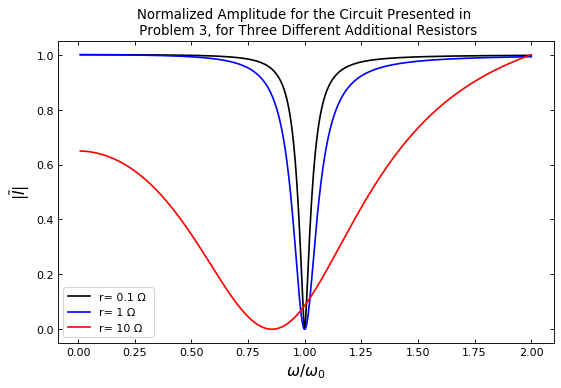
\includegraphics[width = 0.8\linewidth]{PHYS241_Ass4_Figure2.png}
 					\caption{Plot of the current's amplitude found in Question 3, for three additional resistor configurations $r$. We note that increasing the value for the resistance in return decreases the narrowness at the resonance point. Moreover, there exists a critical value of $r$ for which the corresponding plot starts shifting progressively to the left.}
 				\end{figure}
 				
	\end{document}